%%%%%%%%%%%%%%%%%%%%%%%%%%%%%%%%%%%%%%%%%%%%%%%%%%%%%%%%%%%%%%%%%%%%%%%%
\chapter{Android}
\label{sec:android}
%%%%%%%%%%%%%%%%%%%%%%%%%%%%%%%%%%%%%%%%%%%%%%%%%%%%%%%%%%%%%%%%%%%%%%%%

%=======================================================================
\section{Überblick}
%=======================================================================
Android ist ein Betriebssystems, welches primär für Smartphones und Tablets konzeptioniert ist. Das Betriebssystem basiert auf einen Linux Kernel und wird von der Open Handset Alliance (gegründert von Google) entwickelt \cite{overviewAndroid:singh}. Android ist eine freie Software und das am schnellsten wachsende mobile Betriebssystem. Der Marktanteil von Android ist seit 2014 über 80\% und soll sich auch in den darauffolgenden Jahren bei dieser Prozentzahl halten, wie in der Abbildung \ref{figure:marketshare} zu sehen ist. \\
 
\begin{minipage}{\textwidth} 
	\centering	
	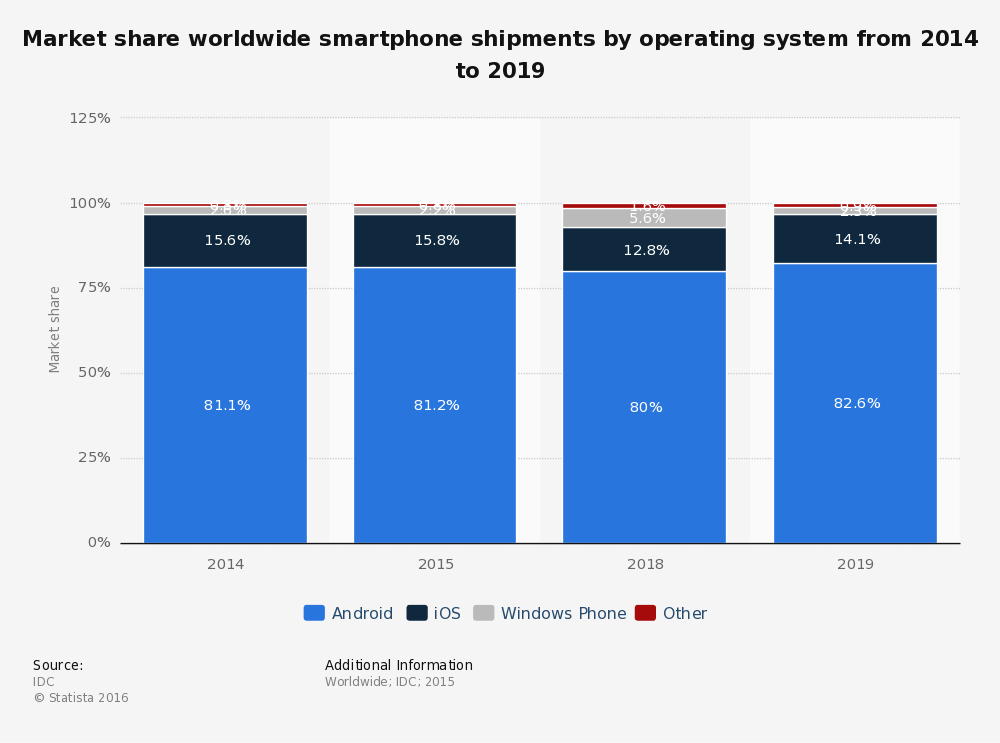
\includegraphics[width=0.65\textwidth]{figures/smartphone-os-market-share.png}
	\captionof{figure}{Marktanteil von mobilen Betriebssystemen \cite{statsticMobileOS}}
	\label{figure:marketshare}
	\vspace{2ex}
\end{minipage}

Durch die quelloffene Struktur des Betriebssystems ist Android bei vielen Konsumenten und Entwicklern sehr beliebt, wodurch Unternehmen ihre mobilen Applikationen auf dieses Betriebssystem ausrichten. Gemäß der Vorhersage von IDC, wird Android zwar eine gewisse Prozentzahl an das Windows Phone Betriebssystem verlieren, aber weiterhin der Marktführer bleiben \cite{statsticMobileOS}.

%=======================================================================
\section{Architektur}
%=======================================================================
Das Android Betriebssystem ist ein Stack von Software Komponenten, welche typischerweise in vier Bereiche gegliedert werden (vgl. \ref{figure:androidArchitekture}). Diese Bereiche sind der Linux Kernel, die Native Bibliotheken, die Laufzeitumgebung, das Application-Framework und die Applikationen \cite{androidTutorialOS}. \\

\begin{minipage}{\textwidth} 
	\centering	
	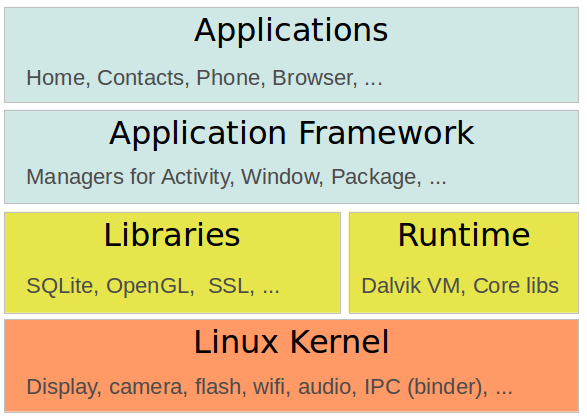
\includegraphics[width=0.65\textwidth]{figures/android_stack.png}
	\captionof{figure}{Android Architektur \cite{androidTutorialOS}}
	\label{figure:androidArchitekture}
	\vspace{2ex}
\end{minipage}

Beschreibung der Software Komponenten der Android Architektur \cite{overviewAndroid:singh}, \cite{androidTutorialOS}: 
\begin{itemize}
	\item \textbf{Applikationen}\\
	Die Applikationen stellen die oberste Schicht der Android Architektur dar. Einige Applikationen sind bereits auf jedem Smartphone vorinstalliert, wie beispielsweise ein SMS Client,  ein Browser oder ein Kontaktmanager. Software Entwickler können ihre eigenen Applikationen schreiben und diese auf dem Smartphone installieren.
	\item \textbf{Application-Framework}\\
    In der Application-Framework-Schicht befinden sich zahlreiche Java-Bibliotheken und Dienste, auf welche Software Entwickler bei der Applikationserstellung Zugriff habe. Wichtige Dienste sind dabei der Activity Manager, der Resource Manager oder der Content Manager.
	\item \textbf{Native Bibliotheken}\\
	Die Nativen Bibliotheken stellen zahlreiche Funktionen für die Application-Framework-Schicht zur Verfügung, wie Grafik-Rendering oder Web-Browsing. Alle diese Bibliotheken sind in C oder C++ geschrieben und werden durch Java Interfaces aufgerufen, bei der Entwicklung von Applikationen.
	\item \textbf{Runtime}\\
	Die Laufzeitumgebung besteht aus der Dalvik Virtual Machine und den Java Kernbibliotheken. Die Dalvik Virtual Machine ist eine Java Virtual Machine, welche speziell für Android entwickelt und optimiert wurde.  Durch die  Dalvik VM kann jede Applikation in einem eigenen Prozess ausgeführt werden, mit einer eigenen Instanz der Dalvik VM. \\
	Durch die Java Kernbibliotheken in der Laufzeitumgebung können Software Entwickler Android Applikationen mithilfe der Programmiersprache Java entwickeln.   
	\item \textbf{Linux Kernel}\\
	Der Linux Kernel stellt die unterste Schicht der Android Architektur dar, welcher leicht von Google abgeändert wurde. Der Kernel ist dabei die Schnittstelle zur Geräte Hardware (Kamera, Display etc.) und ist gleichzeitig für die Speicher- und Prozessverwaltung verantwortlich.
	
	
	
	
	
	
	
	
	
	
	
	
	
	
	
	
	
	
	
	
	
	
	
	
	
	
	
	
	
	
	
	
	
	
\end{itemize}